%\section{Constraints}
%The constraints in this project could fall into two groups. The first constraint is related to the limitation on laboratory conditions \cite{Connor2018BiometricFeatures}. In real-world circumstances, many situations such as walking speed, clothing, footwear, and load carriage could affect our results, whereas our datasets could cover some of these real-world conditions. For example, except for the walking speed and footwear, both datasets do not have useful information for other real-world situations. Consequently, our results are optimistically biased. Table \ref{tab:1_vul} indicates some inhibiting factors. 

%Another significant limitation in the Stepscan dataset is the lack of relative footprint location. The dataset included only aligned and segmented footprint images. The location of samples concerning each other is unknown. This information could play a significant role in predicting the location of future footsteps. 

%\begin{center}
%	\begin{table}[!t]
%	\caption{Some inhibiting factors in gait recognition.}
%	\label{tab:1_vul}
%	\hspace{3em}
%	\setlength\extrarowheight{-2pt}
%	\begin{tabular}{rl}
\toprule
    &  Inhibit Factors \\
\midrule
  1 & Footwear               \\
  2 & clothing               \\
  3 & Injury                 \\
  4 & Muscle development     \\
  5 & Fatigue                \\
  6 & Age                    \\
  7 & Load carriage          \\
  8 & Walking speed          \\
  
\bottomrule
\end{tabular}


%	\end{table}
%\end{center}
 

%\section{Remaining Work}

%In recent years, improvements in the computational process of computers and other benefits of \gls{dnn} have caused many researchers (like \cite{IsmailFawaz2019DeepReview} and \cite{Costilla-Reyes2018DeepSensors}) to move towards \gls{dnn} for the classification of time series data. Therefore, these algorithms will be reviewed in a later stage of this project.

%Because the entire time series were considered for extracting features, we have had one value for each attribute. For instance, while local maximums could be good features, the algorithm returned only the global maximum as a Max feature. We could slide a window on the signal to extract handcrafted features. It causes only a part of the data to consider in each moment. In other words, because each data includes several stages of the walking cycle, features should be extracted according to these periods.   

%Moreover, cropping the heel or toe area in each video could separate features based on the walking stages (pressure area). By this means, each video will be divided into N sub-area, and then for each region, we reconstruct time-series signals and extract features. As a result, these features belong only to that area or stage of walking.

%Due to using the aligned video, we could consider some pixels over time as 2D signals. Although our features space increased rapidly, we could put a threshold on variance and energy of time-series signals for controlling features space. 

%In this research, regardless of eliminating high-correlated and low variance features, we should use a more complex feature selection algorithm to eliminated irrelevant and redundant ones. This reduction might increase the accuracy.

%In addition, it had better to split the dataset into left and right footprints for exploring the effects of extracted features on classifier accuracy. 
 

\section{Experimental Results}
The biometrics industry has utilized two performance measurements, False Rejection Rate (FRR) and False Acceptance Rate (FAR), for accuracy. These measures also are called False Negative Rate (FNR) and False Positive Rate (FPR) in biometric literature. According to these values, a graphical ROC curve was produced by plotting FPR on the x-axis against 1–FNR on the y-axis. Figure \ref{fig:ROC} shows the ROC curves for different models and features. 

The area under the ROC curve (AUC) shows the performance of verification systems. An AUC of 0.5 represents a system with no discriminating ability (The blue line in figure \ref{fig:ROC}), whereas an AUC of 1.0 represents a test with perfect discrimination. Moreover, many researchers often use equal error rate (EER) as an additional metric to describe the performance of biometric systems. EER refers to the point that FRR equals FAR. The smaller value of EER shows the Better performance of the model. Results of four different machine learning algorithms in several types of features are shown in table \ref{tab:1_ML}.


For the training scenario, the first 50 users were used for developing models while other users set aside as imposter data. Then for each subject, a model was trained based on 80 percent data (about 16 in-class samples and 16 $\times$ 49 $\approx$ 780 from impostors class). For testing, A set of four genuine samples and 4 $\times$ 49 $\approx$ 190 from impostor samples were used. Due to the fact that we developed a model for each subject, we averaged FPR and FNR for each method.

The SVM classifier’s best AUC was 91.3\%, as shown in table \ref{tab:1_ML}. This result was come from classifying the combination of all features and the best AUC among all approaches. Other algorithms had similar performance on all features. All kinds of features had the worst results on Random Forests Classifiers. In terms of the EER metric, the SVM classifier achieved the smallest value (about 0.147) on all handcrafted features.









%The SVM performed best with the mixture of all features, at 56\% accuracy (see table \ref{tab:1_ML}). All other feature subsets achieved lower than this amount. The worst performance for all these classifiers belonged to the random forest classifier with about 30\%.



%The area under the ROC curve (AUC) is a global measure of the ability of a test to discriminate whether a specific condition is present or not present. An AUC of 0.5 represents a test with no discriminating ability (ie, no better than chance), while an AUC of 1.0 represents a test with perfect discrimination. The (unpublished) ROC curve for ACS (figure 1) which was generated from the T-MACS scores calculated for the derivation set has an AUC of 0.94 after correction for in-sample optimism by cross-validation, which would suggest that T-MACS score is a very good discriminator of ACS versus no ACS.


 


\begin{center}
	\begin{table}[!t]
	\centering
	\caption{The EER and AUC metric for Machine learning models implemented in this paper.}
	\label{tab:1_ML}
	%\hspace{-1em}
%	\setlength\extrarowheight{-2pt}
	\begin{tabular}{llll}
\toprule
{} &  Frame Work &    AUC &    EER \\
\midrule
0  &     LDA\_ALL &  0.884 &  0.202 \\
1  &    LDA\_SPEC &   0.87 &  0.193 \\
2  &    LDA\_STAT &  0.877 &  0.206 \\
3  &    LDA\_TEMP &  0.881 &  0.215 \\
4  &     LDA\_VGG &   0.75 &  0.306 \\
5  &  LDA\_MOBNET &  0.766 &  0.298 \\
6  &     KNN\_ALL &  0.841 &  0.202 \\
7  &    KNN\_SPEC &  0.811 &  0.228 \\
8  &    KNN\_STAT &  0.822 &  0.206 \\
9  &    KNN\_TEMP &  0.819 &  0.222 \\
10 &     KNN\_VGG &  0.606 &  0.418 \\
11 &  KNN\_MOBNET &   0.63 &  0.404 \\
12 &     SVM\_ALL &  0.913 &  0.147 \\
13 &    SVM\_SPEC &  0.606 &  0.412 \\
14 &    SVM\_STAT &  0.741 &  0.306 \\
15 &    SVM\_TEMP &  0.883 &  0.203 \\
16 &  SVM\_MOBNET &   0.76 &  0.286 \\
17 &     RFC\_ALL &  0.651 &  0.402 \\
18 &    RFC\_SPEC &  0.598 &  0.441 \\
19 &    RFC\_STAT &  0.565 &  0.465 \\
20 &    RFC\_TEMP &  0.608 &  0.438 \\
21 &     RFC\_VGG &  0.573 &  0.453 \\
22 &  RFC\_MOBNET &  0.586 &  0.452 \\
23 &         FCN &  0.798 &  0.285 \\
\bottomrule
\end{tabular}

	\end{table}
\end{center}

\begin{figure}
     \centering
     \begin{subfigure}[b]{0.45\textwidth}
         \centering
         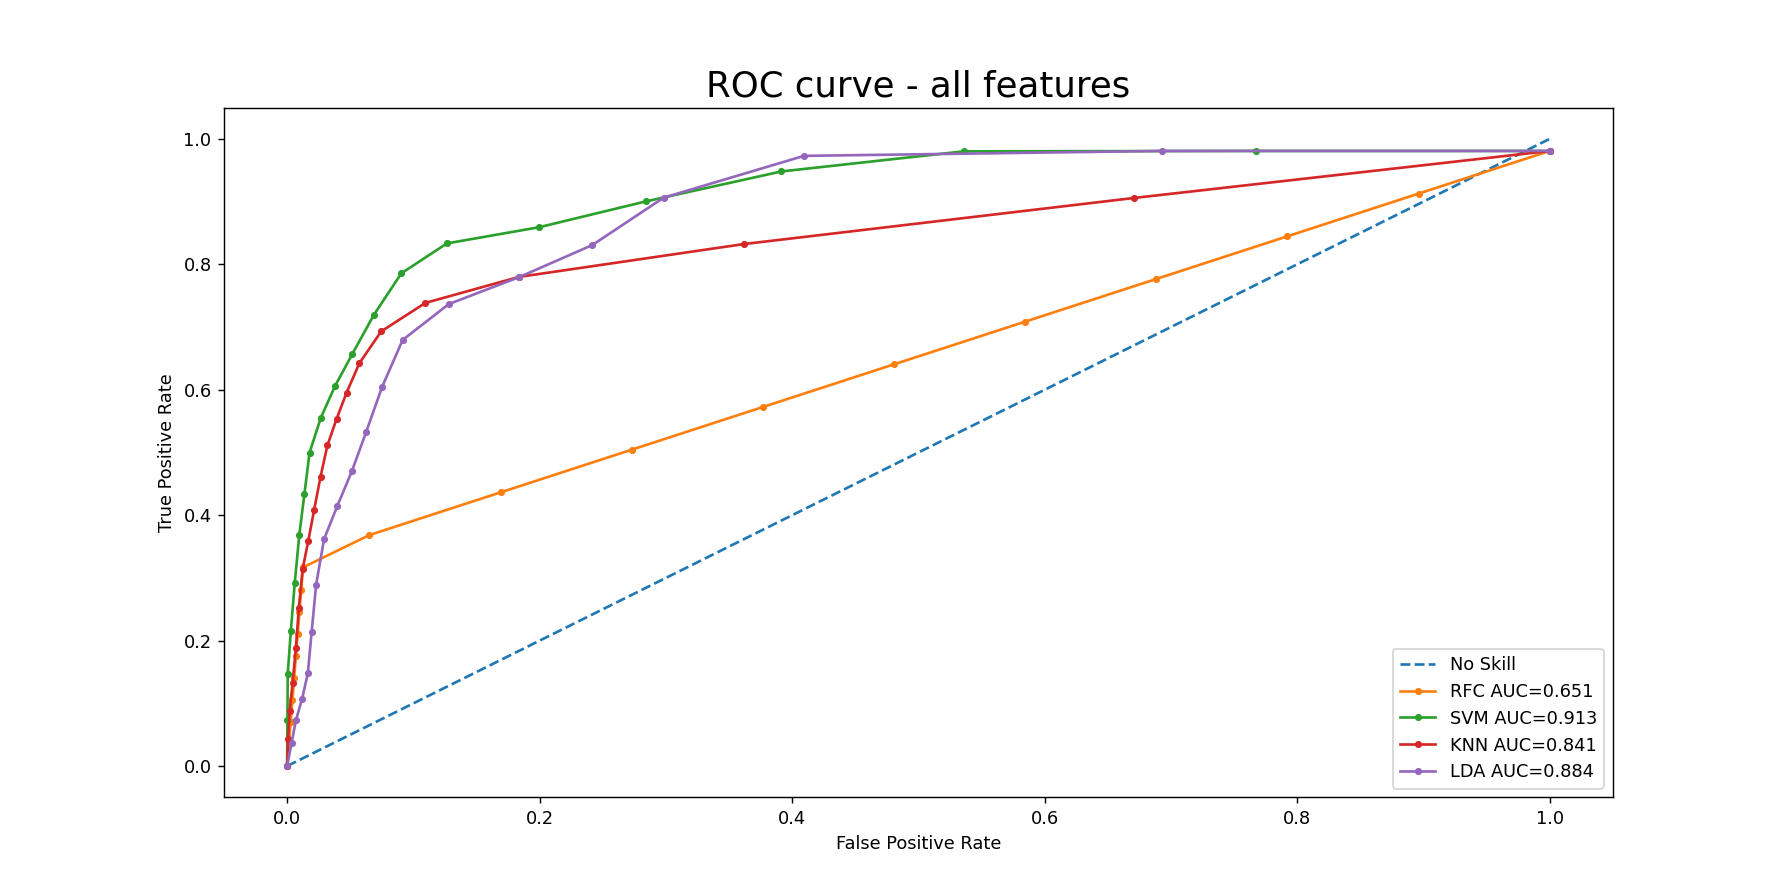
\includegraphics[width=1\textwidth]{manuscript/src/figures/project/roc_curve_all 2021-04-09-11:12:24-tree-Mobnet-standardization.png}
         \caption{The ROC curve of four Machine learning algorithms on handcrafted features}
         \label{fig:ROC_all}
     \end{subfigure}
     \hfill
     \begin{subfigure}[b]{0.45\textwidth}
         \centering
         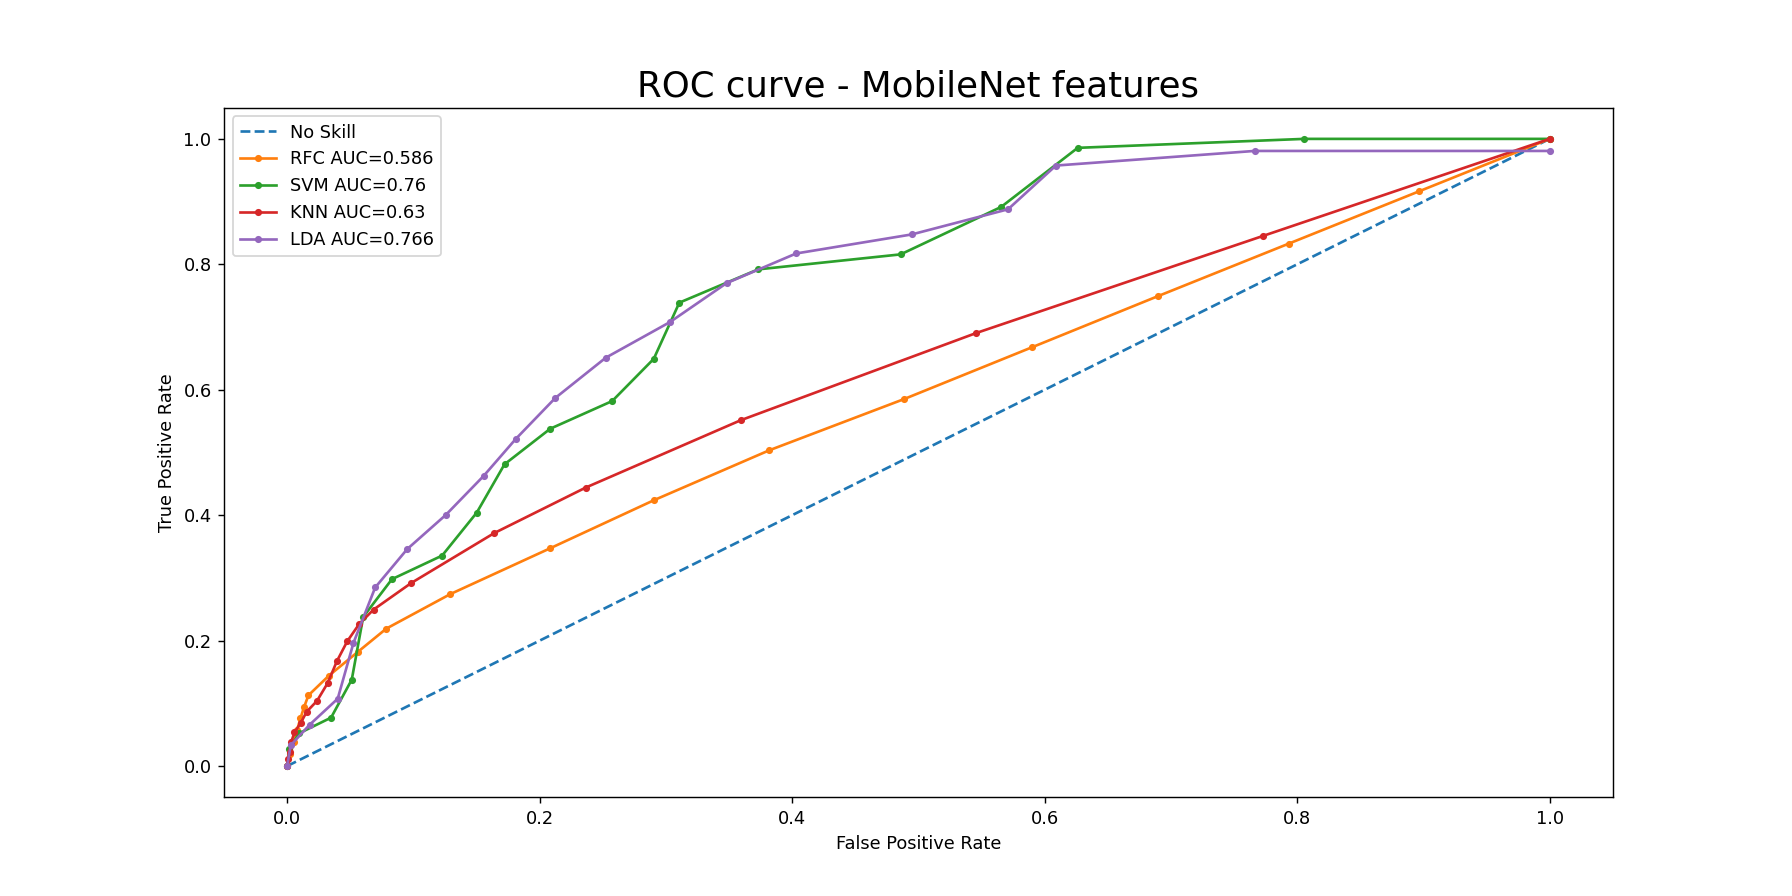
\includegraphics[width=\textwidth]{manuscript/src/figures/project/roc_curve_MobileNet 2021-04-09-11:12:24-tree-Mobnet-standardization.png}
         \caption{The ROC curve of four Machine learning algorithms on MobileNet features}
         \label{fig:ROC_Mob}
     \end{subfigure}
     \vfill
     \begin{subfigure}[b]{0.45\textwidth}
         \centering
         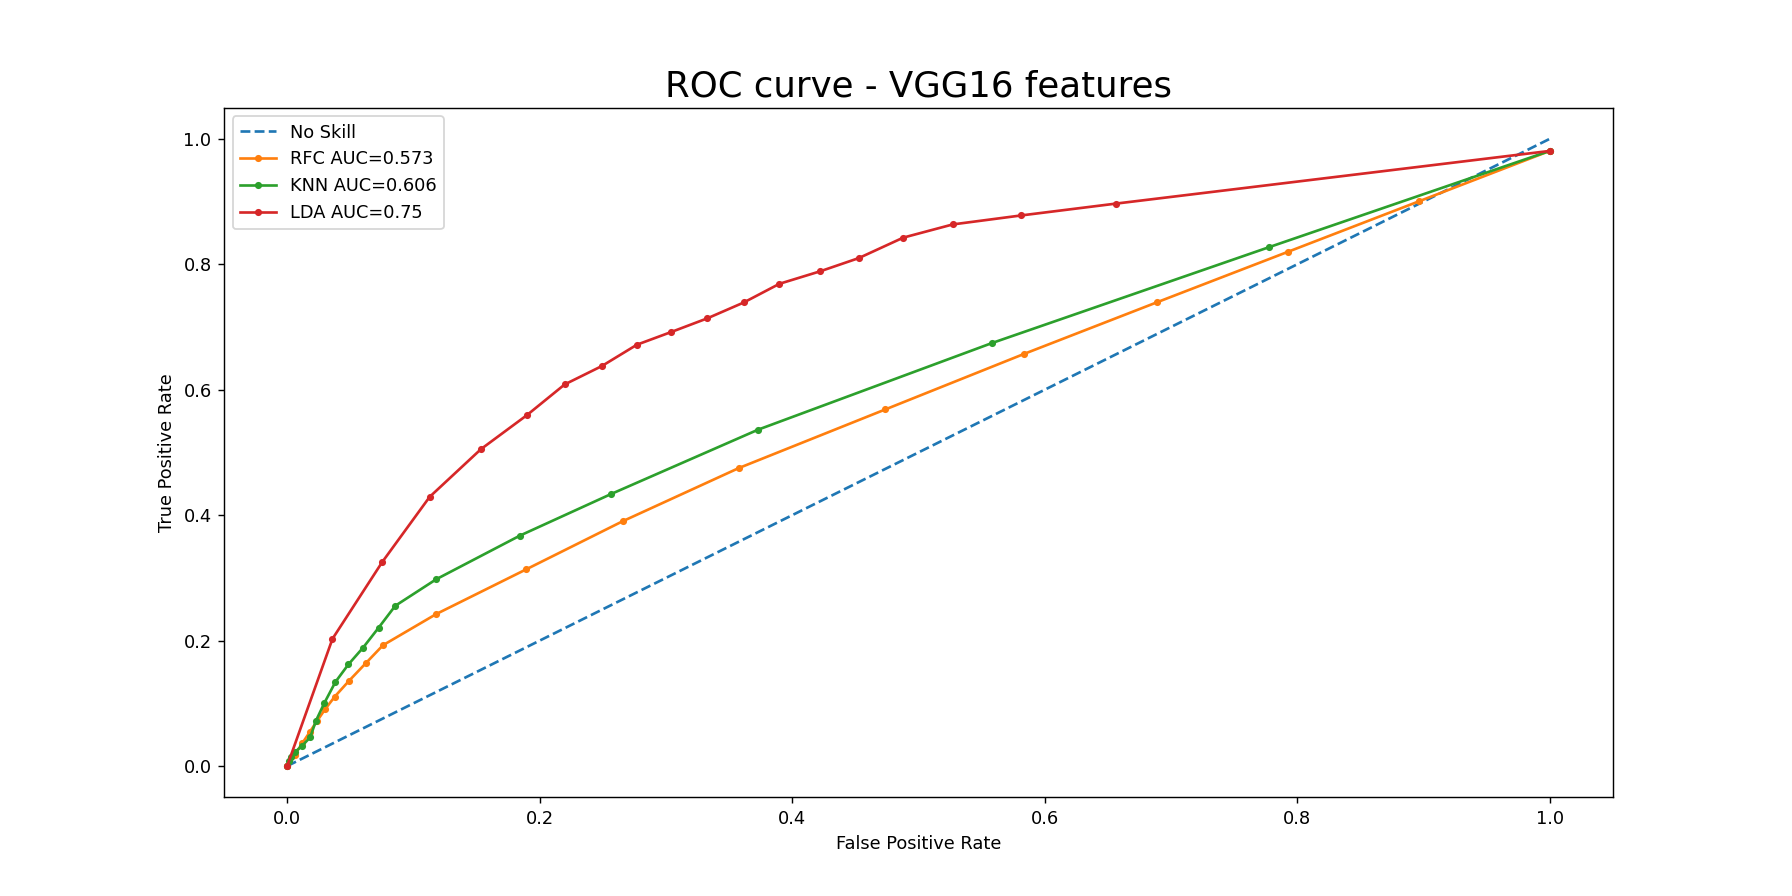
\includegraphics[width=\textwidth]{manuscript/src/figures/project/roc_curve_vgg 2021-04-09-11:12:24-tree-Mobnet-standardization.png}
         \caption{The ROC curve of four Machine learning algorithms on VGG16 features}
         \label{fig:ROC_vgg}
     \end{subfigure}
     \hfill
     \begin{subfigure}[b]{.45\textwidth}
         \centering
         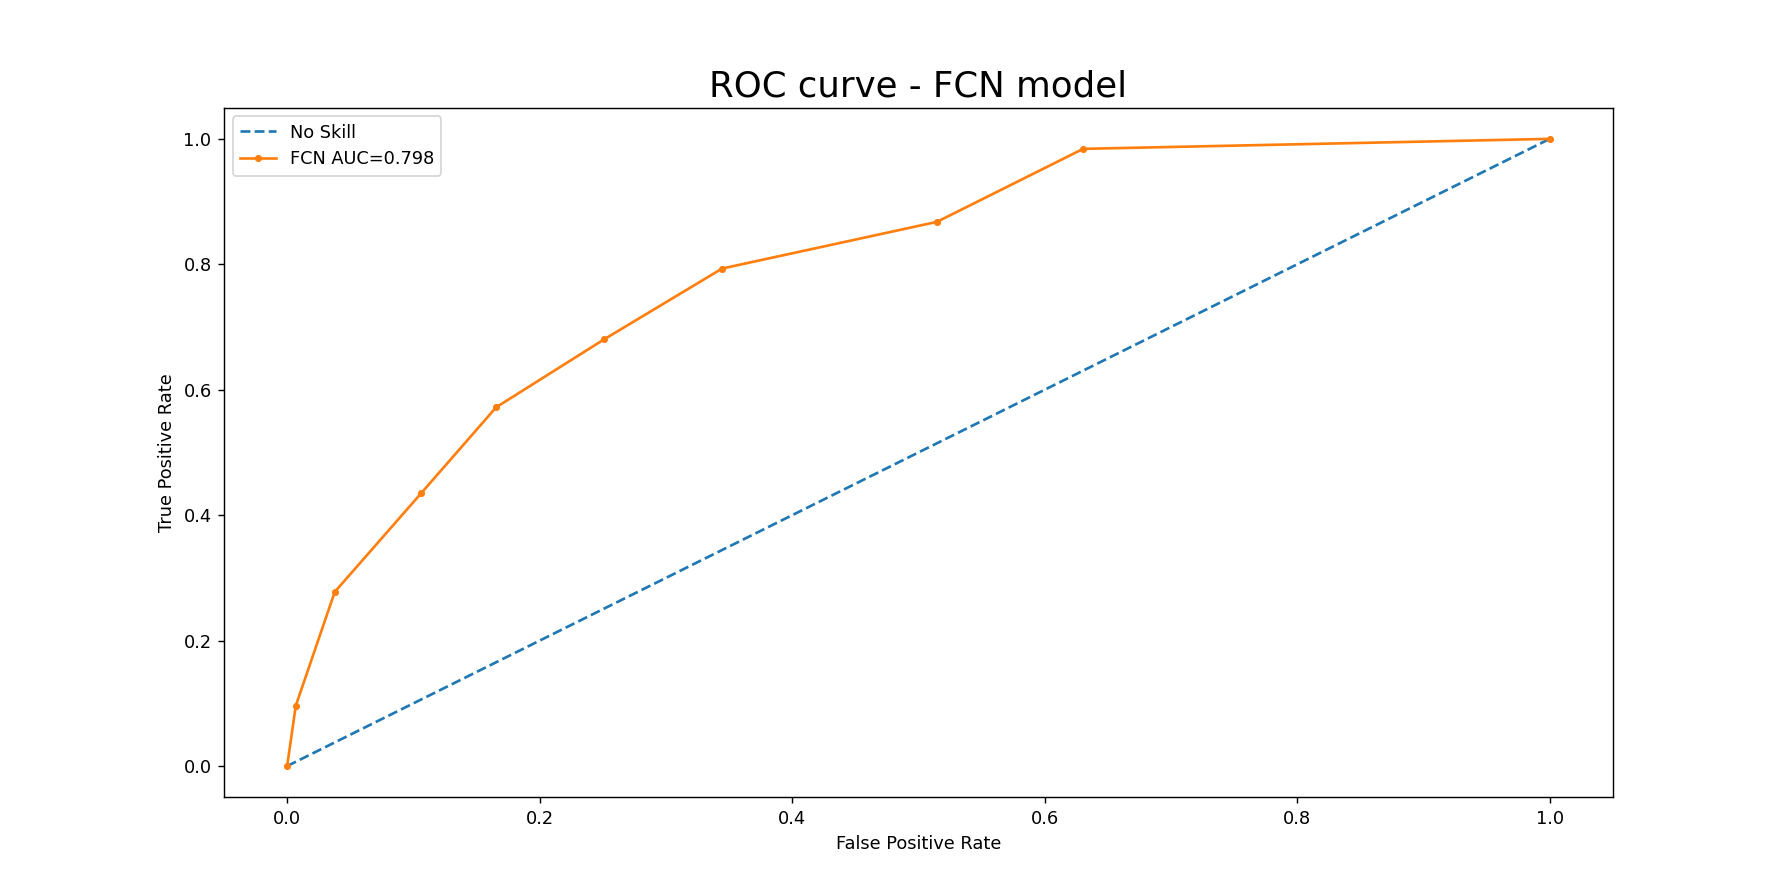
\includegraphics[width=1\textwidth]{manuscript/src/figures/project/roc_curve_FCN 2021-04-09-11:12:24-tree-Mobnet-standardization.png}
         \caption{The ROC curve of Fully Convolutional Network (FCN).}
         \label{fig:ROC_fcn}
     \end{subfigure} 
        \caption{The ROC curve of different approaches}
        \label{fig:ROC}
\end{figure}

%Fig. 9 shows the ROC curves using the test set, indicating that all the hybrid methods achieved higher AUC values than a single conventional classifier. Specifically, the CNN-SVM and CNN-RF methods obtained higher AUC values of 0.868 and 0.829 than SVM and RF, respectively. Furthermore, compared to LR, the CNN-LR method achieved the most significant improvement of 0.063 in terms of AUC. In addition, the AUC value obtained by CNN was higher than single machine learning classifiers, but lower than the hybrid methods. 
